\documentclass[../../main.tex]{subfiles}
\begin{document}


\begin{problem}
\begin{enumerate}
    \item 用 \texttt{LC} 分枝限界算法求解下面的 $0 - 1$ 背包问题，并画出所生成的状态空间树：
          \[
              N = 5, \quad M = 12, \quad (P_1, P_2, \dots, P_5) = (10, 15, 6, 8, 4), (W_1, W_2, \dots, W_5)=(4,6,3,4,2)
          \]

    \item 用 \texttt{FIFO} 分枝限界算法求解下面的 $0 - 1$ 背包问题，并画出所生成的状态空间树：
          \[
              N = 5, \quad M = 15, \quad (P_1, P_2, \dots, P_5) = (W_1, W_2, \dots, W_5) = (4,4,5,8, 9)
          \]
\end{enumerate}
\end{problem}

\begin{solution}
\end{solution}
1. 用 \texttt{LC} 分枝限界
\begin{center}
    \begin{tikzpicture}[scale=0.6]
        \tikzset{every tree node/.style={ draw, rectangle}}
        \Tree
        [.\(1:\hat{c}=-29,u=-25\)
            [.\(2:\hat{c}=-29,u=-25\) [.\(4:\hat{c}=-29,u=-25\) [.\(6:-\) ][.\(7:\hat{c}=-29,u=-25\) [.\(8:-\) ][.\(9:\hat{c}=-29,u=-29\) [.\(10:\hat{c}=-29,u=-29\) ][.\(11:\hat{c}=-29,u=-25\) ]]]][.\(5:\hat{c}=-26,u=-16\) ]][.\(3:\hat{c}=-27,u=-21\) ]
        ]

    \end{tikzpicture}
\end{center}
最优解: \(J = \{1,1,0,0,1\}\), 价值为7.


2. 用 \texttt{FIFO} 分枝限界
\begin{center}
    \begin{tikzpicture}[scale=0.55]
        \tikzset{every tree node/.style={ draw, rectangle}}
        \Tree
        [.\(\hat{c}=-15,u=-13\)
            [.\(\hat{c}=-15,u=-13\)
                    [.\(\hat{c}=-15,u=-13\)
                            [.\(\hat{c}=-15,u=-13\) ]
                                [.\(\hat{c}=-15,u=-8\) ]
                        ] [.\(\hat{c}=-15,u=-9\) ]
                ]
                [.\(\hat{c}=-15,u=-13\) [.\(\hat{c}=-15,u=-9\) ][.\(\hat{c}=-15,u=-13\) [.\(\hat{c}=-15,u=-13\) [.\(\hat{c}=-15,u=-13\) ][.\(\hat{c}=-15,u=-13\) [.\(\hat{c}=-14,u=-14\) ][.\(\hat{c}=-13,u=-13\) ]]][.\(\hat{c}=-15,u=-8\) ]]]
        ]
    \end{tikzpicture}
\end{center}
最优解: \(J = \{0,0,1,0,1\}\), 价值为14.

\end{document}